\documentclass[xcolor={usenames,dvipsnames}]{beamer}

\usepackage[utf8]{inputenc}
\usepackage[T1]{fontenc}

\usetheme[titleformat=regular,numbering=fraction]{metropolis}

\defbeamertemplate*{footline}{shadow theme}
{%
  \leavevmode%
  \hbox{\begin{beamercolorbox}[wd=.5\paperwidth,ht=2.5ex,dp=1.125ex,leftskip=.3cm plus1fil,rightskip=.3cm]{author in head/foot}%
      \usebeamerfont{author in head/foot}\hfill\insertshortauthor
    \end{beamercolorbox}%
    \begin{beamercolorbox}[wd=.5\paperwidth,ht=2.5ex,dp=1.125ex,leftskip=.3cm,rightskip=.3cm plus1fil]{title in head/foot}%
      \usebeamerfont{title in head/foot}\insertshorttitle%
  \end{beamercolorbox}}%
  \vskip0pt%
}

\usepackage{amsmath,amsfonts,amssymb}
\usepackage{mathpartir}
\usepackage{biblatex}
\usepackage{tikz}

\usepackage{bussproofs}
\EnableBpAbbreviations{}
\alwaysRootAtTop{}

\title{mSAT: an OCaml SAT Solver}
\author{Guillaume Bury}
\institute{Université Paris Diderot; \inria{}; LSV, ENS Cachan}
%\date{11 March, 2016}


\begin{document}

\begin{frame}
  \frametitle{A modular, proof producing SAT Solver}

  \begin{itemize}
    \item SAT Solver \textbf{library} in pure OCaml
    \item Make you own SMT Solver thanks to \textbf{functorized design}
      \begin{itemize}
        \item More expressive than pure SAT Solvers (minisat, sattools, ...)
        \item More flexibility than Full SMT Solvers (Alt-ergo-zero, ...)
      \end{itemize}
    \item Proof generation:
      \begin{itemize}
        \item Resolution tree in OCaml, with graphviz output
        \item \textbf{Formal proof} in Coq (and soon Dedukti).
      \end{itemize}
  \end{itemize}
  \hspace*{-1cm}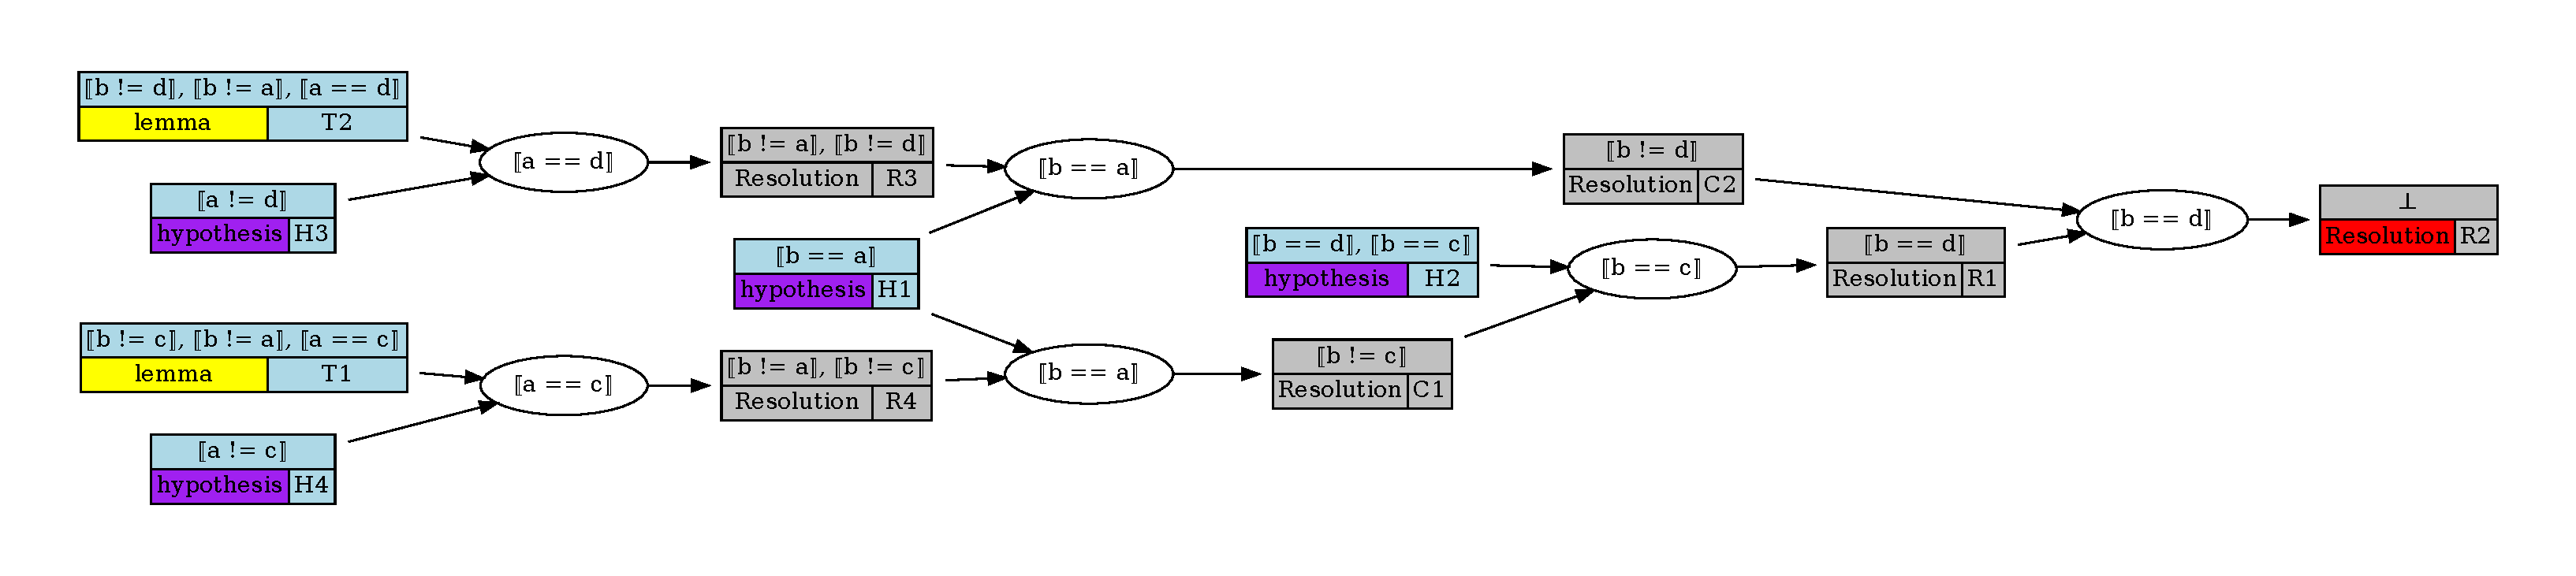
\includegraphics[width=13cm]{proof}
  \begin{itemize}
    \item Performances : Alt-ergo-zero $\overset{x10}{>}$ mSAT $\overset{x10}{>}$ minisat
  \end{itemize}

\end{frame}

\end{document}
